\documentclass[conference,letterpaper]{IEEEtran}

\usepackage[margin=1in]{geometry}
\usepackage{graphicx}
\usepackage{subcaption}
\usepackage{fixltx2e}
\usepackage{gensymb}
\usepackage{todonotes}
\usepackage{url}
\usepackage{amsmath}
\usepackage{amsfonts}
\usepackage{amssymb}
\usepackage{amsthm}
\usepackage{mathtools}
\usepackage{mathrsfs}
\usepackage[ruled]{algorithm2e}

\newcommand\prn[1]{\left( #1 \right)}
\newcommand\bkt[1]{\left[ #1 \right]}
\newcommand\set[1]{\left\{ #1 \right\}}
\newcommand\abs[1]{\left| #1 \right|}
\renewcommand\epsilon{\varepsilon}
\newcommand\aaa{\boldsymbol{a}}
\newcommand\ee{\boldsymbol{e}}
\newcommand\RR{\mathbb{R}}
\newcommand\yy{\boldsymbol{y}}
\newcommand\hfirst{{h_{\mathrm{first}}}}
\newcommand\hlast{{h_{\mathrm{last}}}}
\DeclareMathOperator*{\argmax}{\arg\!max}

% correct bad hyphenation here

\hyphenation{op-tical net-works semi-conduc-tor top-ology}


\begin{document}

%%%%%%%%%%%%%%%%%%%%%%%%%%%%%%%%%%%%
% paper title
%%%%%%%%%%%%%%%%%%%%%%%%%%%%%%%%%%%%
% can use linebreaks \\ within to get better formatting as desired
\title{A Brief Comparison of Algorithms for Detecting Change Points in Data}

%%%%%%%%%%%%%%%%%%%%%%%%%%%%%%%%%%%%
% author names and affiliations
%%%%%%%%%%%%%%%%%%%%%%%%%%%%%%%%%%%%
% option 1)
%%%%%%%%%%%%%%%%%%%%%%%%%%%%%%%%%%%%
% use a multiple column layout for up to three different
% affiliations

\author{\IEEEauthorblockN{Cody Buntain}
\IEEEauthorblockA{Department of Computer Science \\
University of Maryland\\
College Park, MD 20742\\
cbuntain@cs.umd.edu}

\and

\IEEEauthorblockN{Christopher Natoli}
\IEEEauthorblockA{Department of Statistics\\
University of Chicago\\
5801 S Ellis Ave, Chicago, IL 60637\\
chrisnatoli@gmail.com}

\and

\IEEEauthorblockN{Miroslav \v{Z}ivkovi\'{c}}
\IEEEauthorblockA{Institute of Informatics\\
University of Amsterdam \\
1012 WX Amsterdam, Netherlands\\
m.zivkovic@uva.nl}
}

% for over three affiliations, or if they all won't fit within the width
% of the page, use this alternative format:
% 
%%%%%%%%%%%%%%%%%%%%%%%%%%%%%%%%%%%%
% option 2)
%%%%%%%%%%%%%%%%%%%%%%%%%%%%%%%%%%%%
%\author{\IEEEauthorblockN{Maria T. Patterson\IEEEauthorrefmark{1},
%Minnie Mouse\IEEEauthorrefmark{2},
%Mickey Mouse\IEEEauthorrefmark{2}, 
%Pluto\IEEEauthorrefmark{2}\IEEEauthorrefmark{3}}
%
%\IEEEauthorblockA{\IEEEauthorrefmark{1}Center for Data Intensive Science\\
%University of Chicago,
%Chicago, IL 60637\\ mtpatter@uchicago.edu}
%\IEEEauthorblockA{\IEEEauthorrefmark{2}Center for Animated Character Scientists\\
%Chicago, IL 60637}
%\IEEEauthorblockA{\IEEEauthorrefmark{3}NASA Goddard Space Flight Center\\
%Greenbelt, MD 20771}
%}


%%%%%%%%%%%%%%%%%%%%%%%%%%%%%%%%%%%%
% make the title area
%%%%%%%%%%%%%%%%%%%%%%%%%%%%%%%%%%%%
\maketitle
\thispagestyle{plain}
\pagestyle{plain}

%%%%%%%%%%%%%%%%%%%%%%%%%%%%%%%%%%%%
% Abstract
%%%%%%%%%%%%%%%%%%%%%%%%%%%%%%%%%%%%
\begin{abstract}
%\boldmath
Detecting points in data where the underlying distribution changes is not a new task, but much of the existing literature assumes univariate and independent data, assumptions often violated in real data sets. This work addresses this gap in the literature by implementing a set of change point detection algorithms and a test harness for evaluating their performance and relative strengths and weaknesses in multi-variate data of varying dimension and temporal dependence. We then apply our implementations to real-world data taken from structural sensors placed on laboratory a bridge and two years of Bitcoin market data from the Mt. Gox exchange. Though more work is necessary to explore these real-world data sets more thoroughly, our results demonstrate circumstances in which an online, non-parametric algorithm does and does not perform as well as offline, parametric algorithms and provides an early foundation for future investigations.

\end{abstract}
% IEEEtran.cls defaults to using nonbold math in the Abstract.
% This preserves the distinction between vectors and scalars. However,
% if the conference you are submitting to favors bold math in the abstract,
% then you can use LaTeX's standard command \boldmath at the very start
% of the abstract to achieve this. Many IEEE journals/conferences frown on
% math in the abstract anyway.

% no keywords

% For peer review papers, you can put extra information on the cover
% page as needed:
% \ifCLASSOPTIONpeerreview
% \begin{center} \bfseries EDICS Category: 3-BBND \end{center}
% \fi
%
% For peerreview papers, this IEEEtran command inserts a page break and
% creates the second title. It will be ignored for other modes.
\IEEEpeerreviewmaketitle


%%%%%%%%%%%%%%%%%%%%%%%%%%%%%%%%%%%%%%%%%%%%%%%%%%%%%%%%%%%%%%%%%%%%%%
%% INTRODUCTION
%%%%%%%%%%%%%%%%%%%%%%%%%%%%%%%%%%%%%%%%%%%%%%%%%%%%%%%%%%%%%%%%%%%%%%
\section{Introduction}

In many applications where monitoring plays a role (Internet, smart energy grids, reservoir engineering), it is crucial to be able to detect points in time in which anomalies occur (indicating potential failures or attacks). 
This task often involves multidimensionality (more than one sensor) with dependence between sensors and time.
Many of the well-known anomaly detection methods, however, assume one-dimensional and independent input. 
These assumptions are of course too unrealistic in many cases, and straightforward application to more complex problems frequently leads to erroneous results. 
Dependence is thus a common characteristic of multidimensional data (measurement). 
There exist several generic models known to have good capabilities to model data originating from multidimensional and dependent measurements, especially multidimensional autoregressive, moving average (ARMA) time series models, which are popular in econometrics research.
Existing literature on machine learning techniques show that violated model assumptions do not necessarily obviate the efficacy of a given algorithm.
As such, the research documented herein compares three algorithms for detecting change points, two of which are parametric and make assumptions of the underlying data, and the third is non-parametric and does not try to model underlying data distributions.
Additionally, our investigation focuses on multidimensional data that exhibit ``abrupt'' change points and can include multiple change points over time.

We start by giving a short overview of generic models for multidimensional data in Section 2, describing in particular the multidimensional ARMA processes. 
Then we will give a literature overview of change point detection methods for time series data, focusing in particular on multidimensional data, in Section 3. 
From this overview we will describe the methods we have chosen to implement in more detail in Section 4. 
Section 5 then covers the comparative performance among the algorithms we implemented before we close in Section 6.

\section{Generic Models For Multidimensional Time Series Data}

\label{section:genericmodels}
\subsection{Auto-Regressive Moving Average (ARMA) models}
\subsubsection{One-dimensional ARMA}
We will start our overview with one-dimensional ARMA model, which will be then generalized to the multidimensional one in Section~\ref{section:varma}

The Auto-Regressive (AR) model is a random process that describes the behavior of a variable in terms of its own past values. The $p$th-order auto-regressive or AR($p$) process is defined by:
\begin{equation*}
Y_t = \mu + \gamma_1Y_{t-1} + \gamma_2Y_{t-2} + \hdots + \gamma_pY_{t-p} + \epsilon_t,
\end{equation*}
where $\mu$ is an intercept, $Y_{t-1},\hdots,Y_{t-p}$ are the lag values of the variable $Y_t$, and $\gamma_1,\hdots,\gamma_p$ the corresponding parameters,
while $(\epsilon_t)_t$ is a white noise sequence, also known as innovation or error term.

Next, consider the symmetrical model: the $q$th-order Moving Average or MA($q$) process is described by the following equation:
\begin{equation*}
Y_t = \mu + \epsilon_t \theta_1\epsilon_{t-1} - \theta_2\epsilon_{t-2} - \hdots - \theta_q\epsilon_{t-q},
\end{equation*}
where $\mu$ is an intercept, $\epsilon_{t-1},\hdots,\epsilon_{t-p}$ are the lag values of the innovation $\epsilon_t$, and $\theta_1,\hdots,\theta_q$ the corresponding parameters. 

Many (stationary) time series processes can be represented in either an auto-regressive or moving average form. Furthermore, researchers have found that a combination of both forms, that is, the Auto-Regressive Moving Average process (ARMA), has proven to be quite effective in modelling many real-life data sets~\cite{BORCDAV2009}. The ($p,q$)th-order Auto-Regressive Moving Average or ARMA($p,q$) process is given by:
\begin{eqnarray*}
Y_t = \mu + \gamma_1Y_{t-1} + \gamma_2Y_{t-2} + \hdots \\
+ \gamma_pY_{t-p} + \epsilon_t - \theta_1\epsilon_{t-1} - \theta_2\epsilon_{t-2} - \hdots - \theta_q\epsilon_{t-q}.
\end{eqnarray*}

For the discussion on applicability of ARMA model, along with the important conditions like stationarity, invertibility or causality the reader is referred to ~\cite{BORCDAV2009}

The models discussed above can only be applied to stationary data. However, a non-stationary data series can often be transformed into a stationary one by 
taking first differences, that is, by subtracting $Y_{t-1}$ from $Y_t$. A non-stationary series that becomes stationary after being first differenced $d$ 
times is referred to as integrated of order $d$, denoted by $I(d)$. An $I(1)$ series in its un-differenced form will typically be constantly growing, while 
an $I(2)$ series is growing at an ever-increasing rate. Series that are $I(3)$ or greater are extremely unusual, but they do exist. 

Using this insight, the ARMA models defined above can be generalized to be able to deal with non-stationary series. The resulting model is denoted an 
Auto-Regressive Integrated Moving Average model, or ARIMA($p, d, q$). Let $L$ be a lag operator such that $LY_t = Y_{t-1}$. In full, the model is then 
denoted by
\begin{eqnarray*}
\Delta^dY_t = \mu + \gamma_1\Delta^dY_{t-1} + \gamma_2\Delta^dY_{t-2} + \hdots \\
+ \gamma_p\Delta^dY_{t-p} + \epsilon_t - \theta_1\epsilon_{t-1} - \theta_2\epsilon_{t-2} - \hdots \\
- \theta_q\epsilon_{t-q},
\end{eqnarray*}
where
\begin{eqnarray*}
\Delta^d Y_t = (1 - L)^dY_t.
\end{eqnarray*}

\subsubsection{The Multivariate Auto-Regressive Moving Average (VARMA) model}\label{section:varma}
Let $(Y_t)_t$ be the observation vectors, having dimensions $r$. Further, define $z^{-i}$ as a backward shift operator: $z^{-i}Y_t = Y_{t-i}$ for all $i \in \mathbb{N}_+$. Then, the vector auto-regressive moving average model has a form:
\begin{equation}\label{VARMA}
A(z)Y_t = c + B(z)\epsilon_t, 
\end{equation}
where $A,B$ are polynomial matrices in the backward shift operator $z^{-i}$:
\begin{align*}
A(z) &= I_r - \sum_{i=1}^{p} A_i z^{-i}\\
B(z) &= I_r - \sum_{j=1}^q B_j z^{-j} \\
\end{align*}
where $A_i,B_j$ are $r \times r$ matrices, $c$ is a $r$-dimensional constant vector, $(\epsilon_t)_t$ is a $r$-dimensional vector white noise sequence with covariance matrix $R$ and $I_r$ is $r$-dimensional identity matrix. VARMA can model at the same time a dependency with respect to time index for a certain observation $Y^k_t$ but also a dependency across the observations $Y^k_t, Y^l_t$.

The series $Y_t$ is stationary if $|A(x)| \neq 0$ for all $|x| =1$ and it is unit-root non-stationary if $|B(1)| = 0$. Assuming there is no input vector, the 
auto-regressive representation of model~\eqref{VARMA} is given by $\Pi(z)Y_t = \epsilon_t$, where $\Pi(z) = B(z)^{-1}A(z) = I - \sum_{i=1}^{\infty} \Pi_i z^{-
i}$. Note that the second equality only holds under the assumption that $A_0 = B_0 = I$. Under the same assumptions, we also have the moving-average 
representation, $Y_t = \Psi(z)\epsilon_t$, where $\Psi(z) = I + \sum_{i=1}^{\infty} \Psi_i z^{-i}$ is defined by $A(z)\Psi(z) = B(z)$.

\section{Related Work}

In this section we give a general overview of the methods of anomaly detection for multidimensional models, not necessary limiting ourselves only to the 
models described in Section~\ref{section:genericmodels}. We focus here on a particular class of anomaly detection known as \textit{change point detection}. A 
change-point in a time series (a data set with a time component) is a moment in which the underlying probability
distribution changes. This means that we focus on data that evolve over time, showing sudden  and insistent changes at one (or multiple) points in time.   
The aim is to detect when a null hypothesis $H_0$ is rejected, where $H_0$ assumes no changes occur in distribution, or in a specific part of the 
distribution.  For instance, certain methods focus on detecting changes in mean, or change in variance. The point is not only to detect the \textit{existence}
 of such a change point, but also its location (in time). There are quite a lot of different methods for change point detection in the literature, each with 
their own assumptions on the time series.
The emphasis found in the literature is often put on one-dimensional time series, but our main focus will be multidimensional, as well as possible dependence 
\textit{between} time steps. A good survey for different techniques of detecting change points in multidimensional time series   is given in \cite{BANI}.

 The most widely used change point detection methods, also for the multivariate case, are CUSUM and GLR algorithms and their derivatives.

\subsection{CUSUM} \label{CUSUM}
CUSUM stands for Cumulative Sum. The basic CUSUM method detects shifts in mean for independent sequences in the 1-dimensional case, where the densities before and after the change are assumed to be known. 
There are many useful extensions to the basic CUSUM method; we mention several here, but for a broader overview see \cite{BANI}. We first briefly describe the basic CUSUM method. Assume $(X_i)_{i=0}^n$ is a 1-dimensional time series. We consider the following two hypotheses:

\begin{itemize}
\item Null-hypothesis $H_0$: the $X_i (i = 0,\ldots, n)$ are i.i.d. realizations of
a random variable with density $f$.
\item Alternative hypothesis $H_1(k)$: there is a $1\leq k \leq n$ such that the observations are i.i.d. samples from a distribution with density
$f$ up to $k-1$, while from observation $k$ on they are i.i.d. with a different density $g$.
\end{itemize}

The basic CUSUM method is an online method, meaning that every time new observations are coming in, the possibility of a change point is checked. The log likelihood ratio (LLR) is used to compute the test statistic:
$t_n := \max_{k\in\{1,\ldots,n\}} S_{k,n}$, where $S_{k,n} = \sum_{i=k}^n \log(\frac{g(X_i)}{f(X_i)})$. 
For a given threshold $c$, the CUSUM method raises an alarm for the first $n_0$ for which $t_{n_0}>c$.\vskip 0,2cm

The authors of \cite{HTHW} found that so-called \emph{multi-chart CUSUM} to perform better in detecting shifts in mean than the original CUSUM but to be less 
computationally expensive than the original GLR (see below). The multi-chart CUSUM consists of several basic CUSUM charts with different reference values 
that are used simultaneously to detect the mean shift. For example, let the anticipated interval of the mean shift, $\theta$, be in $[a,b]$. Then, we can 
create a CUSUM multi-chart with a number of CUSUM charts $T_C(\varrho_1),\ldots,T_C(\varrho_m)$ by choosing the parameters $\varrho_1,\ldots,\varrho_m$ in 
the interval. If one of the CUSUM charts triggers a mean shift, the CUSUM multi-chart would send an alarm.
%Rowlands et al. (1982) and Sparks (2000) have shown that two or three CUSUMs were sufficient to almost achieve the optimal envelope. 
An optimal design of the CUSUM multi-chart is provided in \cite{HTHW}.\vskip 0,2cm

Also, the CUSUM methodology has been applied to multidimensional problems. A multivariate version of CUSUM, the \emph{MCUSUM}, is given in \cite{HEALY} (see \cite{RPROJ} for the example of implementation). The method is sensitive to small and moderate shifts. In \cite{HEALY} two examples are discussed: 
\begin{itemize}
\item	shift in mean of multivariate normal (MCUSUM reduces to a set of univariate CUSUMs),
\item	shift in covariance for multivariate normal.
\end{itemize}
The method requires tuning to the size of the shift and should only be used if the mean of the anomalous state (or at least its direction compared to 
non-anomalous state) is known. If the specified direction of the shift is wrong, performance can be bad.
% (Methods to overcome this problem are complicated, see e.g. Hawkins and Olwell 1989).

Independence between timesteps is assumed in the previous. In \cite{galeano2007covariance} a CUSUM procedure is introduced for detecting covariance changes in multivariate ARMA processes, so with possible dependence between time steps.
 
While in the previous framework the assumption is made that pre- and post-change densities are known, Tartakovsky \emph{et al.} \cite{TRS} propose a nonparametric (pre- and post-change densities are unknown) multi-chart CUSUM to  detect a change in one out of $N$ independent populations each consisting of a possibly dependent sequence of random variables (the \emph{MNPA-CUSUM}). 
Since in the nonparametric case the log-likelihood ratio (LLR) cannot be computed, the authors suggest to replace them by some `appropriate' score functions that have a negative mean before the changepoint and a positive mean after the changepoint. In this case the CUSUM type statistic remains close to zero or slightly negative in normal conditions while after a changepoint it is drifting upward until it crosses a certain threshold. Indeed, score functions can be chosen in many ways, and their selection depends crucially on the type of change that we intend to detect. For example, different score functions are used to detect changes in the mean and changes in the variance. Tartakovsky \emph{et al.} do not explain how to choose the score function in general, but give an example for detection of abrupt change in mean (other parameters can also change but are treated as nuisance parameters). Pre-change mean values $\mu_i$ of observed data are assumed to be known (or at least estimated accurately) in advance (but should be re-estimated once in a while). Post-change mean values $\theta_i$ should be estimated on-line or pre-set to a reasonable number, depending on the applications (see end of Section 3.1 in \cite{TRBK} for more details and concrete examples). \vskip 0,2cm
In \cite{AUE}, \emph{a non-parametric} version of CUSUM is introduced that can be used to  detect (multiple) changes in the covariance structure of multidimensional, possibly non-linear time series. The authors consider the null hypothesis
$$H_0: \text{Cov}(Y_1)=\ldots=\text{Cov}(Y_n),$$
where ($Y_j,j=1,\ldots,n$) is a sequence of $d$-dimensional random vectors with finite first and second moments where the mean is constant over time. As the 
alternative hypothesis the authors specify
$$H_0: \text{Cov}(Y_1)=\ldots=\text{Cov}(Y_k)\neq \text{Cov}(Y_{k+1})=\ldots=\text{Cov}(Y_n).$$
The asymptotic null distribution is related to the Brownian bridge after rescaling, from which thresholds can be computed.

In \cite{WIED2012} a non-parametric CUSUM-like method is described for detecting changes in correlation matrices for multidimensional time series data with 
some possible dependence. The thresholds are computed via Brownian bridges.


In \cite{ARNOLD} a test is described for detecting change in correlation between two random variables $X_t$ and $Y_t$, so for the bivariate setting. The 
bivariate vector $(X_t, Y_t)$ is assumed to have finite first four moments, and some serial dependence is allowed. In a higher dimensional setting, this test 
might be applied for each of the pairs, leading to $d(d-1)/2$ different tests in the $d$-dimensional case. Similar as in \cite{AUE} the asymptotic null 
distribution is related to the Brownian bridge after rescaling:  $\sup_{0\leq z\leq 1} |B(z)|$.

In \cite{MATTESON} a method is described for performing multiple change point analysis of a sequence of multi-
variate observations. They are able to consistently detect any type of distributional change, and do not make any assumptions beyond the existence of the 
a-th absolute moment, for some $a\in (0,2)$. In this setting however, the assumption must be made that the observations are independent \textit{between} 
timesteps.

In a quite similar setting, \cite{LUNG}  proposed a non-parametric method for offline detection of multiple change points in multivariate data; here as well 
different types of distributional changes are described, and independency between time steps is assumed.

Next we briefly mention other types of methods for anomaly detection encountered in the literature.

\subsection{Generalised Likelihood Ratio}\label{GLR}
Generalised Likelihood Ratio (GLR) was developed in \cite{SIVE} but is also explained in [\cite{BANI}, Section 2.4.3]. A `classic' CUSUM algorithm assumes 
that the distribution after a change point (just like the one before the change point) is fully specified, i.e., not only its form but also all the 
parameters are known. In practice this can often be found unrealistic, thus a change point detection method which can deal with unknown parameters
after a change is desirable. The idea behind a Generalised Likelihood Ratio (GLR) method is to replace unknown parameters in the log-likelihood ratio by 
their maximum likelihood estimators. In [\cite{BANI}, Section~2.4.3] one can find further details of GLR method, along with the assumptions on the 
distributions class for which it can be applied.

A non-exhaustive list of recent developments on GLR will now follow.
\begin{itemize} 
\item In \cite{LAI1995} the reader finds recursive window-limited GLR algorithms for {\bf State Space Models, ARX, Regression Models}. Alternatively see 
[\cite{BANI}, Chapter 7] for how to bring these models back to the multidimensional i.i.d. Gaussian i.i.d.
\item There are also promising modifications for the GLR to account for the (possibly nonparametric) {\bf multivariate} case (see \cite{BANI}).
\item There is no convenient recursive form for the basic GLR which can therefore be computationally complex. Therefore, \cite{WIJO} suggest to use limiting 
windows in the context of detecting additive changes in linear state-space models (see also \cite{LAI2001}, pp. 319). 
\item Also \emph{window-limited GLR} involves many likelihood-ratio computations at each stage. Therefore, \cite{NIKO} establish a new suboptimal recursive 
approach which is based on a collection of L parallel recursive $\chi^2$ tests instead of the window-limited GLR scheme. This new approach involves only a 
fixed number L of likelihood-ratio computations at each stage. According to the authors, by choosing an acceptable value of non-optimality, the designer can 
easily find a trade-off between the complexity of the quadratic change detection algorithm and its efficiency.
\item Tuning problems (window size, threshold,...) have been addressed in ~\cite{LAI1995} and~\cite{LAISHAN1999}
%\item Window-limited GLR can also be extended to non-likelihood (see (Lai and Chan 2000b)). 
\item See \cite{LAI2009} for generalization to the case that {\bf pre- and post-change densities are unknown}. 
%\item \cite{LAI2000} also uses limited-window GLR for {\bf diagnosis}.
\end{itemize}

This procedure can be extended easily to the multichannel problem (multiple independent populations of independent sequences) as discussed in \cite{TART08}.

\subsection{Exponentially Weighted Moving Average}\label{EWMA}
In this method, abbreviated as EMWA, the following quantity is monitored (based on observations $Y_t$ for $t=1,\ldots,n$): 
\[EWMA_t = \lambda Y_t +(1-\lambda) EWMA_{t-1}\]
where $EWMA_0$ is assumed to be a historical mean and $\lambda \in (0,1]$
determines `forgetting speed' (amount of the history taken into consideration). An alarm is issued when $EWMA_t$ exceeds a certain threshold.
For details on the \textit{multivariate} exponentially weighted moving average control charts (MEWMA) see \cite{LOWRY} and \cite{PRAB}. This multidimensional 
version has the following properties:
\begin{itemize}
\item assumes that the process follows a (multi-dimensional) normal distribution with known mean and covariance;
\item	is sensitive to small persistent shifts in mean in any direction
\item	for the correlated data, if it is desired to detect small changes in process variability, so-called EWMA V-chart can be used, as proposed in \cite{YEH};
\item	the method requires tuning to the size of the shift;
\item  pre-change distribution must be known.
\end{itemize}
Moreover, \cite{KRSC} proposed a generalization of the MEWMA to the case of multivariate time-dependent observations.

\subsection{ChangeFinder} \label{ChangeFinder}
The \emph{ChangeFinder} is a scheme for detecting outliers and change points  in time series. For details see \cite{TAYA}. The ChangeFinder performs the following steps:

\begin{enumerate}
\item Read data $x_t$. As an example, \cite{TAYA} assume that $x_t$ can be modeled as a {\bf multidimensional AR process}.
\item Learn the probability density $p_t$ (\cite{TAYA} propose an algorithm for doing so in the AR case).
\item Compute the \emph{logarithmic loss score} 
\[score(x_t)=-\log p_{t-1}(x_t|X_1^{t-1}), \]
where $X_1^{t-1}=x_1,\ldots,x_t$ (alternatively they propose the \emph{quadratic loss score} 
\[score(x_t)=\left( x_t-\hat{x}_t\right)^2, \]
where $\hat{x}_t$ is  the prediction value for $x_t$ given $X_1^{t-1}$ based on model $p_{t-1}$). A higher score indicates that $x_t$ is an outlier with higher probability. 
\item Compute $y_t=\frac{1}{T} \sum_{i=t-T+1}^t score(x_i)$, the moving average of the scores.
\item Learn the density $q_t$ of $y_t$ (in the AR case by using the same algorithm as before).
\item Compute $$score(t)=\frac{1}{T}\sum_{i=t-T+1}^t -\log q_{i-1}(y_i|Y_{i-k}^{i-1})$$ A higher score $score(t)$ indicates that time point $t$ is a change point with higher probability. 
\end{enumerate}

The role of the two moving average processes is to reduce the influence of sole outliers. In the case where $T$
is small, outliers and change points can be detected immediately after they appear. However, they may be difficult to discriminate from one another. In the case where $T$ is large, it leads to time delay for detecting change points; however, outliers are filtered and only significant change points are detected accurately.

\subsection{Subspace Identification} \label{Subspace}
By using a pre-designed time-series model a subspace is discovered by principal component analysis from trajectories in past and present intervals, and their 
dissimilarity is measured by the distance between the subspaces. One of the major approaches called subspace identification \cite{KYM}, which compares the 
subspaces spanned by the columns of an 'extended observability matrix' (whose building blocks are the system matrices) generated by a {\bf linear state-space 
model} with system noise. This paper discusses nonparametric
algorithms for change-point detection in time-series data, based on the principle that the subspace spanned by the columns of an extended observability 
matrix is approximately equivalent to the one spanned by the sub-sequences of time-series data. Change-point detection is performed by estimating, on the 
basis of subspace identification, the column space of the extended observability matrix of the SSM behind time-series data, and the evaluating the sub-
sequence of new-arrived data based on this subspace. The authors of \cite{KYM} claim that their method can handle more abundant type of time-series data than 
conventional approaches because of implicitly utilizing generic SSMs, instead of AR models or constrained SSMs, as the model behind time series data.The 
method can explicitly handle interdependence over time. According to \cite{KYM} the algorithm can be implemented easily also for on-line detection, they 
provide some pseudo-code. They also discuss the way their algorithm applies to input-output time-series data.

\subsection{Direct Density Ratio Estimation} \label{DRE}
A common limitation of some of the above mentioned approaches is that they rely on pre-specified parametric models such as probability density models (CUSUM, 
GLR), auto-regressive models and state-space models. As mentioned earlier, to overcome this problem non-parametric method can be used. While non-parametric 
methods usually rely on non-parametric density estimation to calculate the log-likelihood ratio (LLR), in \cite{SUGI2012} the authors suggest to estimate the 
density ratio directly instead of estimating the individual densities and then they show how to use this approach in change-point detection. They use so-
called Kullback-Leibler importance estimation procedure (KLIEP, see \cite{KASU}). Later they extend this method and use methods denoted as
unconstrained least-squares importance fitting (uLSIF) or relative uLSIF (RuLSIF) as building blocks (see \cite{SUGI2012}). The usefulness of the proposed 
method is demonstrated through experiments using artificial and real-world data sets. Furthermore, the dimensionality reduction approach for high-dimensional 
problems discussed in \cite{YASU}. Also, \cite{SUGI2011} provide R and MATLAB implementations for density ratio estimation procedures for outlier detection. 

\subsection{Recipe for on-line changepoint detection}\label{recipe}

 For on-line detection algorithms, the pre-change parameter is supposed to be known as it can be estimated accurately. Let $\theta$ be the parameter after change. Then, concerning this parameter we have to distinguish three cases:
\begin{enumerate}
\item\label{thetaknown}  pre-change parameter $\theta$ is known (or estimated from a training sample).
\item\label{thetahalfknown} we have few information about $\theta$, e.g. it is known that there exists a seperating hyperplane between the old parameter and $\theta$.
\item\label{thetaunknown} nothing is known about $\theta$.
\end{enumerate}

Let $k$ be the time that the change happens. Concerning $k$ we distinguish
\begin{enumerate}[(a)]
\item\label{kunknown} $k$ is a nonrandom unknown value or a random unknown with unknown distribution.
\item\label{kknown} there is some a priori information about the distribution of $k$ 
\end{enumerate}

\section{Implemented Algorithms}

\subsection{Likelihood Ratio Test}

In Galeano and Pe\~{n}a's work on detecting covariances changes in multivariate data, they proposed two methods for calculating test statistics from which change points could be identified \cite{galeano2007covariance}. 
These methods model the given data as a vector autoregressive integrated moving average (vARIMA) popular in economics and financial market analysis, extracting the errors (or innovations) from this data, and applying these methods on this error data.
The first such statistic, on which we focus here, uses a likelihood-ratio test (LRT) to compare two hypotheses: the null hypothesis $H_n$ that the covariance of this error data is best characterized by a single covariance matrix $\Sigma$ versus the alternative hypothesis $H_a$ that, at some time point $h$, the data is best characterized by two separate covariances matrices $\Sigma_1$ before $h$ and $\Sigma_2$ after $h$.
The logarithm of a modified form of the ratio $H_n/H_a$ then generates a test statistic $LR_{h}$ that existing literature shows is governed by a chi-squared distribution with degrees of freedom proportional to the dimensionality $k$ of the data.
From simulations of this distribution, we can generate a critical value given some $\alpha$ against which to compare this test statistic to determine whether a change point actually exists at some time $h$.

\subsubsection{Algorithm}

Given some time-series data $\tilde{y}_t$ and confidence $\alpha$, we use the following algorithm to identify points of change in covariance:

\begin{function}
	\SetAlgoLined
	fit VARIMA$(p, d', q)$ model to $\tilde{y}_t$ \;
	compute residuals $\hat e_t$ \;
	\BlankLine
	$k \gets$ dimension($\tilde{y}_t$) \;
	$d \gets k(p + q + 1) + \frac{k(k+1)}{2} + 1$ \tcc*[r]{minimum points needed} 
	$n \gets$ len$(\tilde{y}_t)$ \;
	$df \gets \frac{k(k+1)}{2}$ \tcc*[r]{degrees of freedom for $\chi^2$} 
	\BlankLine
	$C \gets $ simulateChiSquareMax$(df, \alpha)$ \tcc*[r]{obtain the critical value} 
	\BlankLine
	$LR \gets $ zeros$(n)$ \;
	$S \gets \frac{1}{n} \Sigma_{i=1}^n e_i \cdot e_i'$ \;
	\For{$h \in [d, n-d-1]$}{
		$v \gets h / n$ \;
		$S_1 \gets \frac{1}{h} \Sigma_{i=1}^h e_i \cdot e_i'$ \;
		$S_2 \gets \frac{1}{n-h} \Sigma_{i=h+1}^n e_i \cdot e_i'$ \;
		$LR[h] \gets n \ln \frac{|S|}{|S_1|^v |S_2|^{1-v}}$ \;
	}
	\BlankLine
	$h_{max} \gets argmax_h(LR) $ \;
	$\Lambda_{max} \gets LR[h_{max}]$ \;
	\BlankLine
	changePoints $\gets [\;]$ \;
	\If{$\Lambda_{max} > C$}{
		changePoints += $ h_{max}$ \;
		\BlankLine
		$W \gets$ transformation governing new data regime (see \cite{galeano2007covariance})\;
		changePoints += apply LRT to $\hat{e}_t[0:h_{max}]$ \;
		changePoints += apply LRT to $W \cdot \hat{e}_t[h_{max}+1:n]$ \;
	}
	\BlankLine
	return changePoints
 \caption{LRT($\tilde{y}_t, \alpha$) Algorithm by Galeano and Pe\~{n}a \cite{galeano2007covariance}}
\end{function}

\subsubsection{Implementation Details}

To implement LRT, we used Python and Scikit's statsmodels package for fitting data to VAR() models.
One should note this restriction to VAR() models is a result of an existing constraint in the statsmodels package. 

We also implemented a version of the LRT algorithm that does not rely on calculating the $W$ transformation matrix.
Rather than evaluating $W$, we leveraged statsmodels and its maximum likelihood estimation to fit the data to two new VAR() models for each regime.
The above algorithm performs better than this secondary implementation because it obviates the need for separate rounds of maximum likelihood estimation for each level of recursion.

\subsection{CUSUM}

The following changepoint detection algorithm, which focuses on changes in the covariance matrix, was designed by Galeano and Pe\~{n}a \cite{galeano2007covariance}.

Suppose the $k$-dimensional time series $\yy_t$ can be represented as a VARIMA process
$$\Phi(B)\yy_t=\boldsymbol{c}+\Theta(B)\aaa_t,$$
where $B$ is the backshift operator and the error or innovation $\aaa_t$ is an iid Gaussian random variable with mean $\boldsymbol{0}$ and covariance matrix $\Sigma_i$, where $i$ indicates the particular regime.

The cusum test statistic is derived from accumulating the sum of squared errors. Since we do not know the true errors $\aaa_t$, we first fit a VARIMA process $\hat\yy_t$ to the time series $\yy_t$ and use the residuals $\ee_t=\yy_t-\hat\yy_t$ as estimates for the errors. Consider the interval $\set{\ell,\ldots, r}$. We can estimate the covariance matrix of the time series in this interval by
$$\hat\Sigma_\ell^r=\frac{1}{r-\ell}\sum_{t=\ell}^r\ee_t\ee_t^\top.$$
Denote the sum of squares accumulated up to time $h$ by
$$A_\ell^r(h)=\sum_{t=\ell}^h\ee_t^\top\prn{\hat\Sigma_\ell^r}^{-1}\ee_t,$$
where the squared errors are in some sense normalized by the empirical covariance $\hat\Sigma_\ell^r$ of the entire interval.

The cusum test statistic for a changepoint at time $h+1$ is then
$$C_\ell^r(h)=\frac{h}{\sqrt{2k(r-\ell+1)}}\prn{\frac{A_\ell^r(h)}{h}-\frac{A_\ell^r(r-\ell+1)}{r-\ell+1}}.$$
The term outside the parentheses is another normalization factor. The left-hand term inside the parentheses is the cumulative sum of squares up to time $h$. The right-hand term inside the parentheses is the cumulative sum of squares for the entire interval $\set{\ell,\ldots,r}$. The test statistic $C_\ell^r(h)$ compares these latter two terms. For example, if there is no changepoint in $\set{\ell,\ldots,r}$, then $\frac{A_\ell^r(h)}{h}$ and $\frac{A_\ell^r(r-\ell+1)}{r-\ell+1}$ will be approximately equal. However, if there is a single changepoint at time $t=h+1$, then the left-hand term is the sum of squares for all of the first regime (and only the first regime), while the right-hand term is the sum of squares over the entirety of both regimes. This suggests that the cumulative sums of squares are most different, and thus $C_\ell^r(h)$ is greatest in magnitude, at the changepoint $t=h+1$.

This observation is confirmed by plotting $\abs{C_\ell^r(h)}$ vs. $h$ for simulated data. Therefore, let
\begin{align*}
\Gamma_\ell^r&=\max_{h\in\set{\ell,\ldots,r}}|C_\ell^r(h)|\\
\bar h_\ell^r&=\argmax_{h\in\set{\ell,\ldots,r}}|C_\ell^r(h)|.
\end{align*}
Galeano and Pe\~{n}a prove that $\Gamma_\ell^r$ asymptotically has the distribution of the supremum over $[0,1]$ of a Brownian bridge. This is a known distribution, allowing us to calculate the critical value $C_\alpha$ for any given significance level $\alpha$.

\subsubsection{Algorithm for finding multiple changepoints}

The approach to finding multiple changepoints is similar to binary segmentation. Let $d=k(p+q+1)+\frac{k(k+1)}{2}+1$ be the resolution of the changepoint detection algorithm. First fit a VARIMA model to the data and computing the residuals. Then let $\hfirst=1+d$ and $\hlast=T-d$, the final time step. Search for a changepoint in $\set{\hfirst,\ldots,\hlast}$ by checking if $\Gamma_\hfirst^\hlast$ exceeds the critical value. Let $\bar h_{\mathrm{old}}=\bar h_\hfirst^\hlast$.

If a candidate is found, split the entire time series at the time $t_2=\bar h_{\mathrm{old}}$ of the candidate changepoint. Check $\Gamma_\hfirst^{t_2}$ if greater than the critical value; if so, redefine $t_2$ as $\bar h_\hfirst^{t_2}$. Repeat until $\Gamma_\hfirst^{t_2}$ is no longer significant. This procedure thus finds the earliest point in the time series at which a changepoint could occur. Redefine $\hfirst$ as the last significant value of $\bar h_\hfirst^{t_2}$. Perform the same procedure over the interval $\set{\bar h_{\mathrm{old}},\ldots,\hlast}$, acquiring a new $\hlast$ as the latest point in the time series at which a changepoint could occur. If $\abs{\hfirst-\hlast}<d$, i.e., the resolution of the algorithm is not high enough to distinguish between $\hfirst$ and $\hlast$, then record $\bar h_{\mathrm{old}}$ as a candidate changepoint. Otherwise, record both $\hfirst$ and $\hlast$ as candidate changepoints. Then repeat this procedure in the narrower interval $\set{\hfirst,\ldots,\hlast}$. Thus, rather than continually cutting the interval in two and repeating the procedure in each part, the algorithm instead narrows down the interval in which changepoints can occur, using previous changepoints as the new endpoints of the narrower interval.

The algorithm ends up find excess candidates. To solve this retrospectively, let $x_1=1$, $x_s=T$, and $\set{x_2,\ldots,x_{s-1}}$ be the sorted list of candidate changepoints. In each interval $\set{x_i+1,\ldots,x_{i+2}-1}$, drop $x_i$ from the list of candidates if $\Gamma_{x_i+1}^{x_{i+2}-1}$ is insignificant. Repeat this procedure until convergence. Then remove $x_1$ and $x_s$ from the list of candidate changepoints. Denote the winnowed list of candidates by $X$. Then the final changepoints detected by the algorithm are $\set{x+1:x\in X}$.

The entire procedure is detailed more explicitly in the following algorithm:

\begin{algorithm}
  \nlset{Step 1}fit VARIMA model to $\yy_t$\;
  compute residuals $\ee_t$\;
  $candidates\gets\set{1,T}$\;
  $\hfirst\gets 1+d$;\quad$\hlast\gets T-d$\;
  \While{True}{
    \nlset{Step 2}\eIf{$\Gamma_\hfirst^\hlast<C_\alpha$}{
      break\;
    }{
      $\Gamma_{\mathrm{old}}\gets\Gamma_\hfirst^\hlast$;\quad$\bar h_{\mathrm{old}}\gets\bar h_\hfirst^\hlast$\;
      $\Gamma\gets\Gamma_{\text{old}}$;\quad$\bar h\gets\bar h_{\text{old}}$\;
      \nlset{Step 3a}\While{$\Gamma>C_\alpha$}{
        $t_2\gets\bar h-1$\;
        $\Gamma=\Gamma_{\hfirst}^{t_2}$\;
      }
      $\hfirst\gets t_2$\;
      $\Gamma\gets\Gamma_{\text{old}}$;\quad$\bar h\gets\bar h_{\text{old}}$\;
      \nlset{Step 3b}\While{$\Gamma>C_\alpha$}{
        $t_1\gets\bar h+1$\;
        $\Gamma=\Gamma_{t_1}^{\hlast}$\;
      }
      $\hlast\gets t_1$\;
      \nlset{Step 3c}\eIf{$|\hlast-\hfirst|>d$}{
        append $\hfirst, \hlast$ to $candidates$\;
        $\hfirst=\hfirst+d$;\quad$\hlast=\hlast-d$\;
      }{
        append $\bar h_{\text{old}}$ to $candidates$\;
        break\;       
      }
    }
  }
  sort $candidates$\;
  $\set{x_1,\ldots,x_s}\gets candidates$\;
  \nlset{Step 4}\Repeat{convergence}{
    \For{$i\in\set{1,\ldots,s-2}$}{
      \If{$\Gamma_{x_i+1}^{x_{i+2}-1}<C_\alpha$}{
        remove $x_{i+1}$ from $candidates$\;
      }
    }
  }
  remove $1,T$ from $candidates$\;
  $changepoints\gets\set{x+1:x\in candidates}$\;
 \caption{Cusum algorithm by Galeano and Pe\~na. The four steps correspond to Galeano and Pe\~na's enumeration.}
\end{algorithm}


\subsection{Kernel Change Detection}

Offline, parametric methods for change point detection often outperform their online, non-parametric competitors, but the flexibility gained by looser model restrictions and the ability to run in a streaming context are at times more valuable.
The kernel-based change detection (KCD) algorithm proposed by Desbory et al. is one such online algorithm \cite{1468491}.
Rather than rely on a priori knowledge of the generating distribution for a given series of data, KCD instead leverages support vector machines (SVMs) to construct descriptions of the data in a higher dimensional space defined by some given kernel (for our cases, the radial basis function, or RBF, kernel).
One can then use these high-dimensional descriptions to develop a dissimilarity statistic that characterizes the differences in center and spread of two possible regimes in the data.
Additionally, SVM's popular kernel trick allows one to generate this dissimilarity statistic in input space rather than feature space.

\subsubsection{Geometric Interpretation}

Desobry et al. provide a compelling geometric interpretation of the KCD based on angles between vectors as a measure of dissimilarity and spread (see Figure \ref{fig:kcdGeo} for a two-dimensional view). 
This geometric interpretation exists in feature space and assumes that two one-class SVMs were used to describe data from a possible past regime and a possible future regime respectively. 
The angle between the vectors normal to the decision planes $\widehat{c_pc_f}$ can then be used as a dissimilarity metric between the two sets of data.
To account for within-class spread, the authors then normalize this angle by the sum of the angles between the respective normal vectors a support vector of each regime $\widehat{c_ps_p}$ and $\widehat{c_fs_f}$.
The result is the KCD dissimilarity statistic shown in Eq. \ref{eq:kcd}.

\begin{figure}[htbp]
\begin{center}
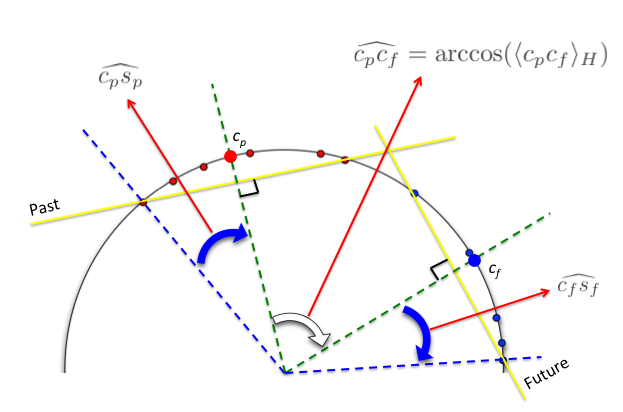
\includegraphics[width=0.5\textwidth]{kcd.png}
\caption{KCD Geometry in Feature Space}
\label{fig:kcdGeo}
\end{center}
\end{figure}

\begin{equation}
\label{eq:kcd}
KCD_{stat} = \frac{\widehat{c_pc_f}}{\widehat{c_fs_f} + \widehat{c_ps_p}}
\end{equation}

These angles can be calculated using the inverse cosine of the dot product between the weight vectors, as shown in Eq. \ref{eq:kcd2}.
One should note the denominator in Eq. \ref{eq:kcd2} is for normalizing the vectors to unit length.
This normalized dot product can be calculated in input space using SVM's learned weights $\boldsymbol{\alpha_p}$ and $\boldsymbol{\alpha_f}$ and the kernel matrices $K$ as shown in Eq. \ref{eq:kcd3}.
To obtain the within-class spread for each class, we use a similar form but rely on the SVM's intercept $\rho$ rather than a dot product, as shown in Eq. \ref{eq:kcd4}.

\begin{equation}
\label{eq:kcd2}
\widehat{c_pc_f} = \arccos \left(\frac{\langle w_p, w_f \rangle_F}{\| w_p \|\| w_f \|} \right)
\end{equation}

\begin{equation}
\label{eq:kcd3}
\frac{\langle w_p, w_f \rangle_F}{\| w_p \|\| w_f \|}  = \frac{\boldsymbol{\alpha}_p^T K_{p, f} \boldsymbol{\alpha}_f }{\sqrt{\boldsymbol{\alpha}_p^T K_{p, p} \boldsymbol{\alpha}_p }\sqrt{\boldsymbol{\alpha}_f^T K_{f, f} \boldsymbol{\alpha}_f }}
\end{equation}

\begin{equation}
\label{eq:kcd4}
\widehat{c_is_i} = \arccos \left(\frac{\rho_i}{\sqrt{\boldsymbol{\alpha}_i^T K_{i,i} \boldsymbol{\alpha}_i }} \right), i \in \{ p, f \}
\end{equation}

\subsubsection{Algorithm}

KCD has four parameters: 

\begin{itemize}
\item $m$ -- Window size, or the number of points on either side of a candidate change point.
\item $\gamma$ -- SVM parameter governing bandwidth for the RBF kernel (other kernels are possible, but we did not experiment with them).
\item $\nu$ -- One-class SVM parameter governing proportion of points that should be counted as outliers when training.
\item $\eta$ -- Threshold parameter such that, if $KCD_{stat} \ge \eta$ for some time point $h$, $h$ is considered a change point.
\end{itemize}

We assume $X$ is the input data of size $n \times k$.

\begin{function}
	\SetAlgoLined
	$n \gets$ len$(X)$ \;
	\BlankLine
	changePoints $\gets [ \; ]$ \;
	\For{$h \in [m, n-m-1]$}{
		$X_{p} \gets X[h-m, h]$ \;
		$X_{f} \gets X[h, h+m]$ \;
		\BlankLine
		svm$_p \gets$ SVM.fit($X_{p}, \gamma, \nu$) \;
		svm$_f \gets$ SVM.fit($X_{f}, \gamma, \nu$) \;
		\BlankLine
		$\boldsymbol{\alpha}_p \gets \text{svm}_p.\alpha$ \;
		$\boldsymbol{\alpha}_f \gets \text{svm}_f.\alpha$ \;
		\BlankLine
		$\boldsymbol{\rho}_p \gets \text{svm}_p.\rho$ \;
		$\boldsymbol{\rho}_f \gets \text{svm}_f.\rho$ \;
		\BlankLine
		$K_{p, p} \gets \text{rbf}(X_p, X_p)$ \;
		$K_{f, f} \gets \text{rbf}(X_f, X_f)$ \;
		$K_{p, f} \gets \text{rbf}(X_p, X_f)$ \;
		\BlankLine
		$\widehat{c_pc_f} \gets \arccos \left(  \frac{\boldsymbol{\alpha}_p^T K_{p, f} \boldsymbol{\alpha}_f }{\sqrt{\boldsymbol{\alpha}_p^T K_{p, p} \boldsymbol{\alpha}_p }\sqrt{\boldsymbol{\alpha}_f^T K_{f, f} \boldsymbol{\alpha}_f }} \right)$ \;
		$\widehat{c_ps_p} \gets \arccos \left(  \frac{ |\boldsymbol{\rho}_p|}{\sqrt{\boldsymbol{\alpha}_p^T K_{p, p} \boldsymbol{\alpha}_p }} \right)$ \;
		$\widehat{c_fs_f} \gets \arccos \left(  \frac{ |\boldsymbol{\rho}_f|}{\sqrt{\boldsymbol{\alpha}_f^T K_{f, f} \boldsymbol{\alpha}_f }} \right)$ \;
		\BlankLine
		$KCD_{stat} \gets \frac{c_pc_f}{c_ps_p + c_fs_f}$ \;
		\If{$KCD_{stat} > \eta$}{
			changePoints += $h$
		}
	}
	\BlankLine
	return changePoints
 \caption{KCD($X, m, \gamma, \nu, \eta$) Algorithm by Desobry et al.\cite{1468491}}
\end{function}

\section{Performance Comparison}

For covariance changes, we generated two regimes of data with constant mean and different covariance matrices. 
KCD then fit one-class SVMs to the covariance matrices within the past and future windows. 
Mean shifts used random means and constant covariance.
We simulated 500 bi-variate data points with a change point at h=250, KCD window size of 400 (m=200), and compared the LRT and CUSUM test statistics at the 95\% confidence level.
Results for this comparison of change point types is shown in Figure \ref{fig:f1ScoresType}.

\begin{figure}[htbp]
\begin{center}
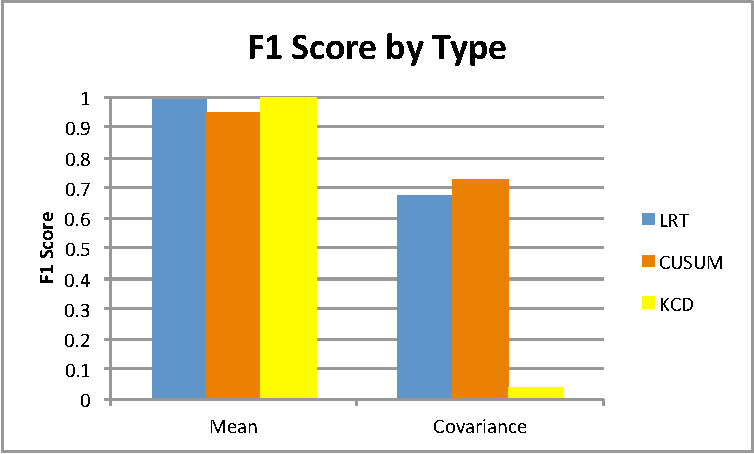
\includegraphics[width=0.5\textwidth]{figures/typeGraph}
\caption{F1 Scores by Type}
\label{fig:f1ScoresType}
\end{center}
\end{figure}

To explore sensitivity to dimensionality, we simulated 500 multi-variate data points but included change points at $h=\{125, 250, 375\}$. 
We left the KCD window size at 400 (m=200), and compared the LRT and CUSUM test statistics at the 95\% confidence level. We then varied dimensionality from $k=[2, 10]$.
Results for both types of change points are shown in Figures \ref{fig:dimensionMean} and \ref{fig:dimensionCov}.

\begin{figure}[htbp]
\begin{center}
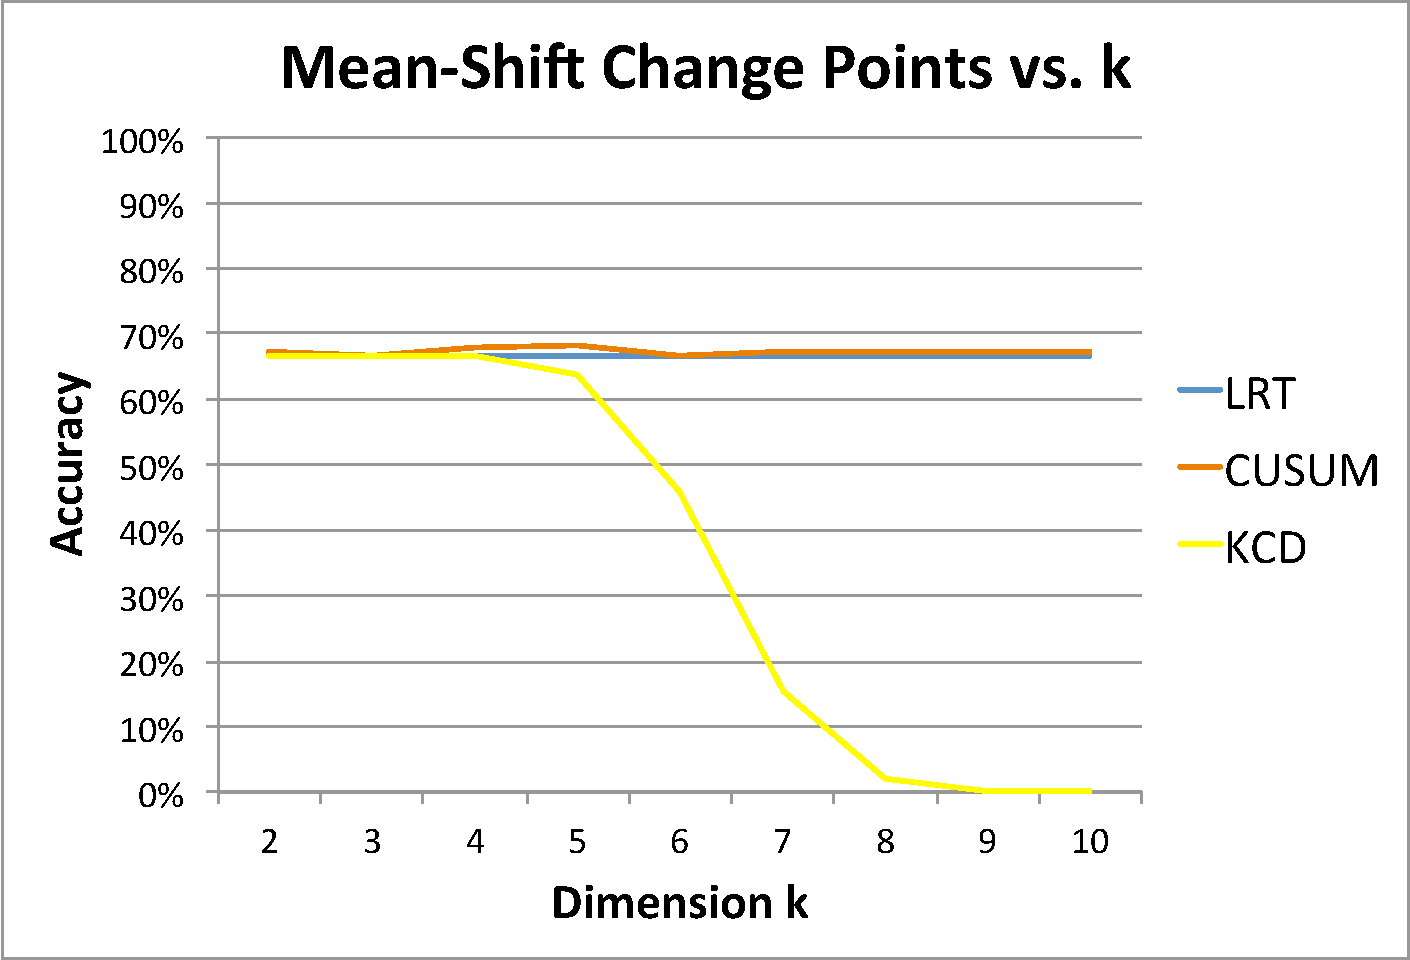
\includegraphics[width=0.5\textwidth]{figures/dimMean}
\caption{Mean-Shift Accuracy versus Dimension $k$}
\label{fig:dimensionMean}
\end{center}
\end{figure}

\begin{figure}[htbp]
\begin{center}
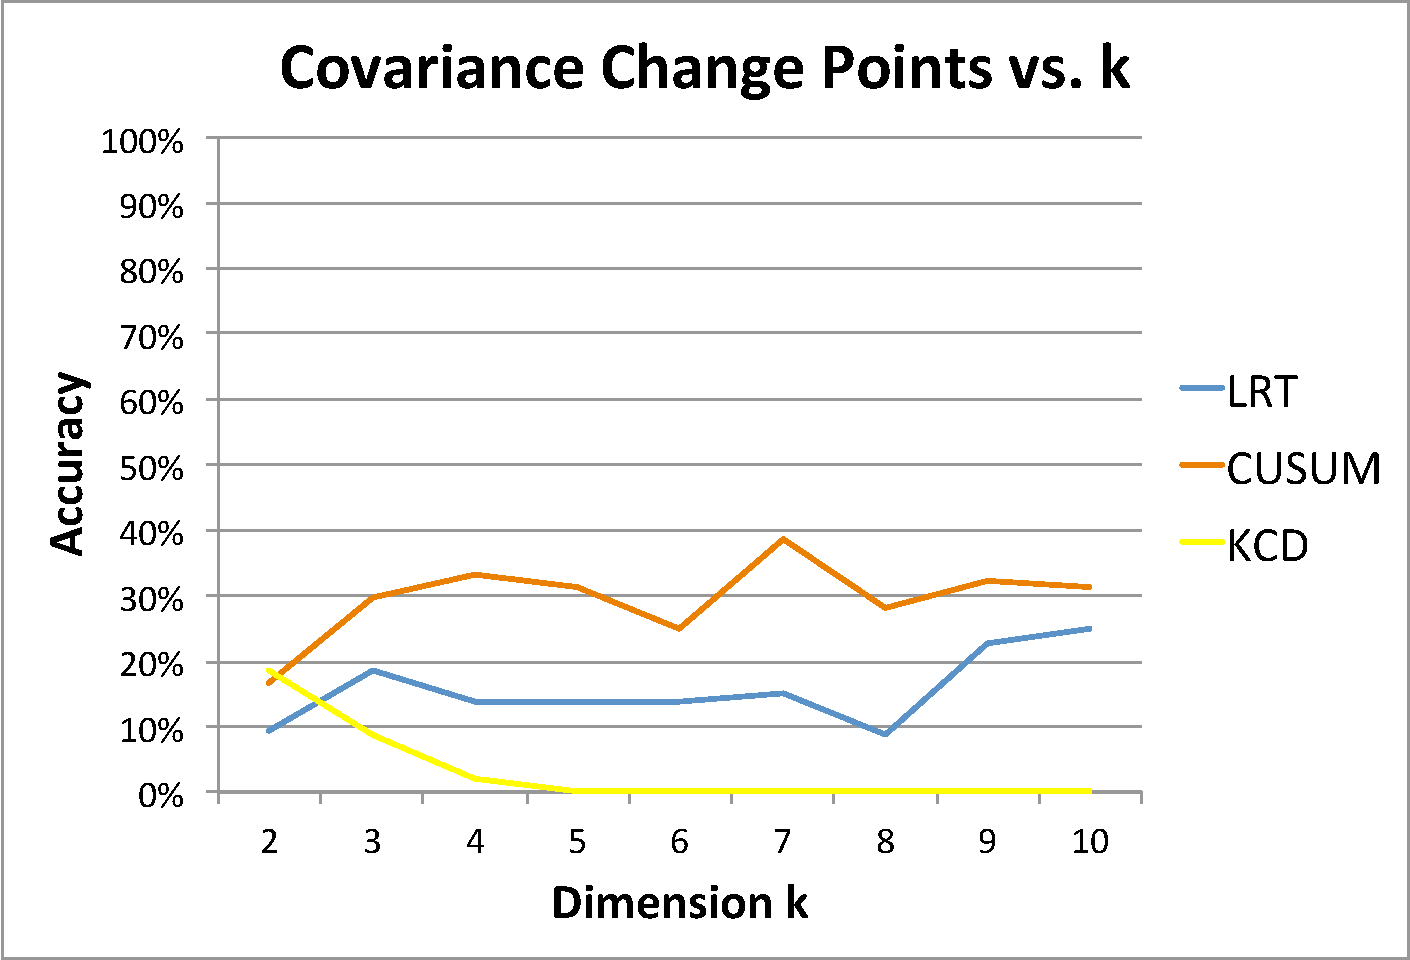
\includegraphics[width=0.5\textwidth]{figures/dimCov}
\caption{Covariance Accuracy versus Dimension $k$}
\label{fig:dimensionCov}
\end{center}
\end{figure}

It seems the LRT and CUSUM-based algorithms are realatively insensitive to increases in dimensionality. KCD, on the other hand, seems quite sensitive with its accuracy falling to near 0\% by $k=9$.

To explore how well these algorithms adapted to multiple change points, we simulated 3,000 bi-variate data points with 2 to 12 change points distributed evenly throughout the data set. 
We left the KCD window size at 400 (m=200), and compared the LRT and CUSUM test statistics at the 95\% confidence level.
Results are shown in Figures \ref{fig:cpMean} and \ref{fig:cpCov}.

\begin{figure}[htbp]
\begin{center}
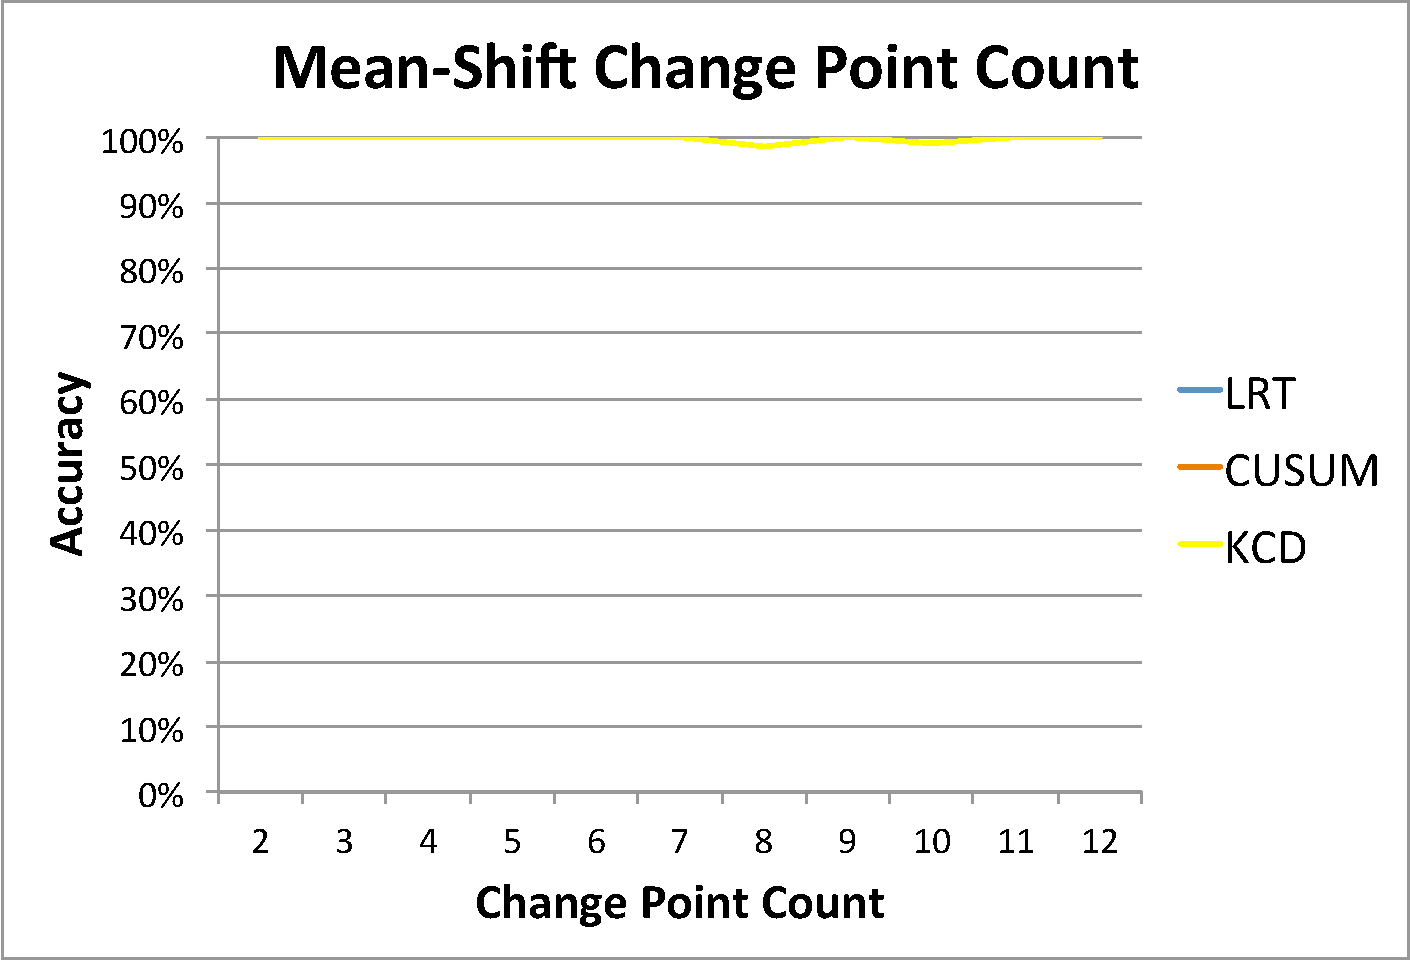
\includegraphics[width=0.5\textwidth]{figures/cpCountMean}
\caption{Mean-Shift Accuracy versus Change Points}
\label{fig:cpMean}
\end{center}
\end{figure}

\begin{figure}[htbp]
\begin{center}
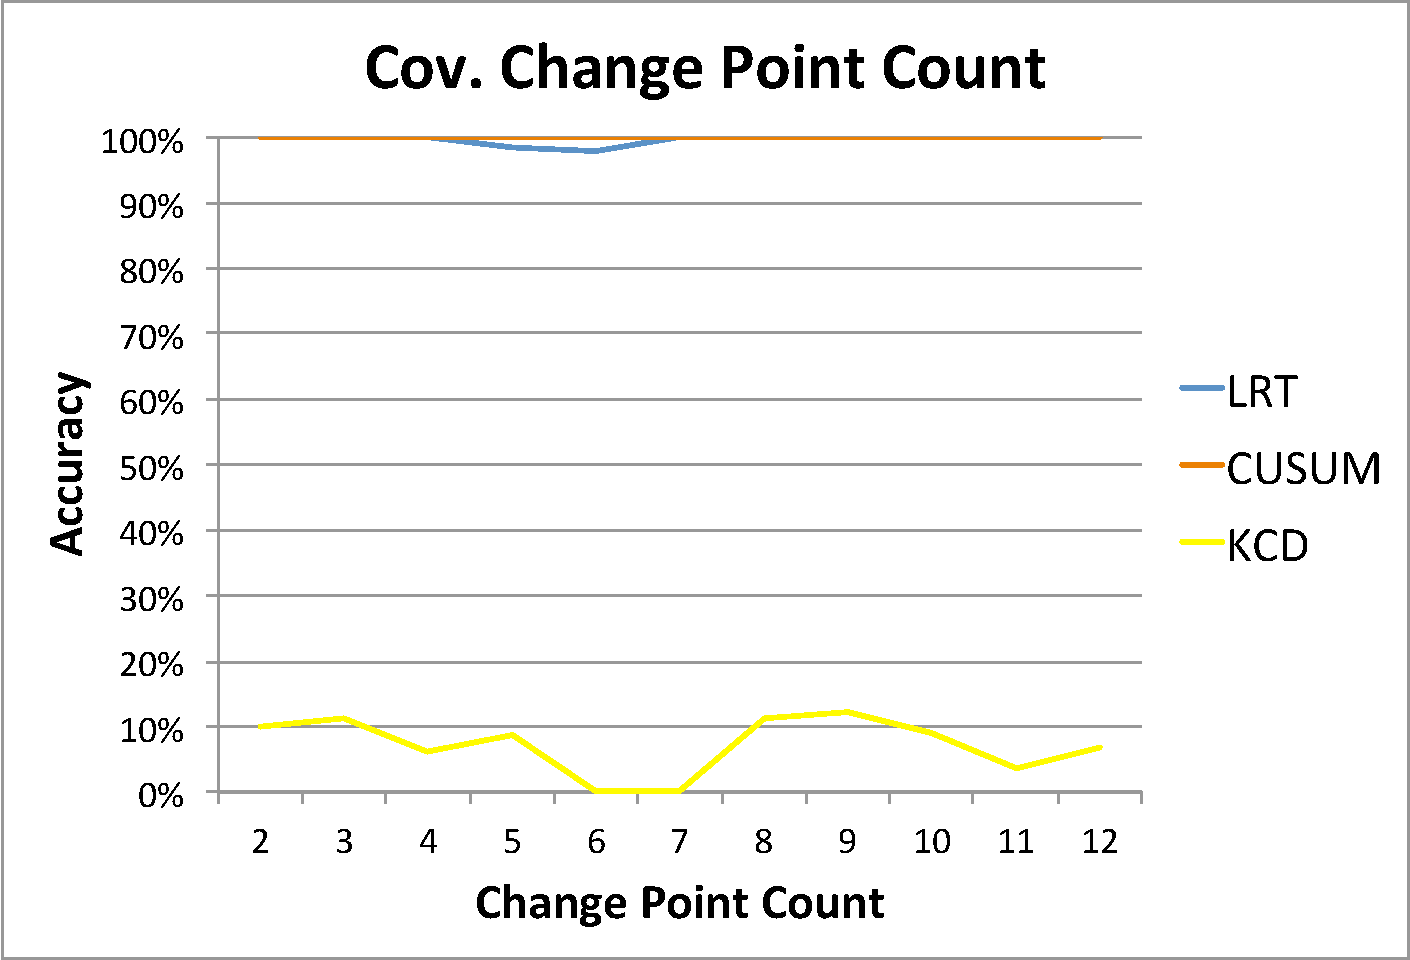
\includegraphics[width=0.5\textwidth]{figures/cpCountCov}
\caption{Covariance Accuracy versus Change Points}
\label{fig:cpCov}
\end{center}
\end{figure}

\section{Conclusions}

Our performance data suggests several interesting results.
First, the parametric LRT and CUSUM algorithms outperform the non-parametric KCD algorithm when detecting changes in covariance.
Second, KCD is competitive in detecting shifts in mean even with relatively small window sizes.
Also, LRT and CUSUM are more robust to increases in dimensionality of the data.

% use section* for acknowledgement
\section*{Acknowledgment}
This work made use of the Open Science Data Cloud (OSDC) which is an Open
Cloud Consortium (OCC)-sponsored project. The OSDC is supported in part by
grants from Gordon and Betty Moore Foundation and the National Science 
Foundation and major contributions from OCC members like the University of 
Chicago.  Both Cody Buntain and Christopher Natoli were supported by the 
National Science Foundation Partnerships for Research and Education (PIRE) 
Award Number 1129076. Any opinions, findings, and conclusions or 
recommendations expressed are those of the author(s) and do not necessarily 
reflect the views of the National Science Foundation. 

This work was made possible using the resources of the Open Science Data Cloud \cite{Grossman2012}.

% references section

% can use a bibliography generated by BibTeX as a .bbl file
% BibTeX documentation can be easily obtained at:
% http://www.ctan.org/tex-archive/biblio/bibtex/contrib/doc/
% The IEEEtran BibTeX style support page is at:
% http://www.michaelshell.org/tex/ieeetran/bibtex/
% argument is your BibTeX string definitions and bibliography database(s)
\bibliography{sources}
\bibliographystyle{IEEEtran}


\end{document}
%%%%%%%%%%%%%%%%%%%%%%%%%%%%%%%%%%%%%%%%%%%%%%%%%%%%%%%%%%%%%%%%%%%%%%%
%% STUFF FROM THE TOP
%% bare_conf.tex
%% V1.3
%% 2007/01/11
%% by Michael Shell
%% See:
%% http://www.michaelshell.org/
%% for current contact information.
%%
%% This is a skeleton file demonstrating the use of IEEEtran.cls
%% (requires IEEEtran.cls version 1.7 or later) with an IEEE conference paper.
%%
%% Support sites:
%% http://www.michaelshell.org/tex/ieeetran/
%% http://www.ctan.org/tex-archive/macros/latex/contrib/IEEEtran/
%% and
%% http://www.ieee.org/

%%*************************************************************************
%% Legal Notice:
%% This code is offered as-is without any warranty either expressed or
%% implied; without even the implied warranty of MERCHANTABILITY or
%% FITNESS FOR A PARTICULAR PURPOSE! 
%% User assumes all risk.
%% In no event shall IEEE or any contributor to this code be liable for
%% any damages or losses, including, but not limited to, incidental,
%% consequential, or any other damages, resulting from the use or misuse
%% of any information contained here.
%%
%% All comments are the opinions of their respective authors and are not
%% necessarily endorsed by the IEEE.
%%
%% This work is distributed under the LaTeX Project Public License (LPPL)
%% ( http://www.latex-project.org/ ) version 1.3, and may be freely used,
%% distributed and modified. A copy of the LPPL, version 1.3, is included
%% in the base LaTeX documentation of all distributions of LaTeX released
%% 2003/12/01 or later.
%% Retain all contribution notices and credits.
%% ** Modified files should be clearly indicated as such, including  **
%% ** renaming them and changing author support contact information. **
%%
%% File list of work: IEEEtran.cls, IEEEtran_HOWTO.pdf, bare_adv.tex,
%%                    bare_conf.tex, bare_jrnl.tex, bare_jrnl_compsoc.tex
%%*************************************************************************
